\documentclass[10pt, twoside]{article}
\usepackage{main}

% Aquí empieza el documento{{{
\begin{document}

%\maketitle
\thispagestyle{fancy}

\textbf{Alberto Oporto Ames: \#139}

\section{Preguntas}%
\label{sec:preguntas}

\begin{enumerate}
	\setcounter{enumi}{3}
	\item ¿Cómo funciona un transformador?
		\subitem Recibe corriente alterna que genera un campo magnético
			variable dentro de un nucleo de hierro.
			Esto genera $Fem$ en el cable enrrollado en el otro extremo.
			Además el voltaje de entrada entre el voltaje de salida es
			proporcional al número de vueltas de entrada entre las de salida.
	\setcounter{enumi}{4}
	\item ¿Para que sirve el galvanómetro y cómo funciona?
		\subitem Para medir campos magnéticos.
			Se hace pasar corriente por unas espiras, y estás giran cuando
			están dentro de un campo magnético.
\end{enumerate}

\section{Problemas}%
\label{sec:problemas}

\textbf{
	En el instante mostrado, se suelta el imán.
	Responde las siguientes preguntas respecto al observador:
}

\begin{figure}[H]
	\centering
	\begin{tikzpicture}[scale=1, transform shape]
		\foreach \y / \p in {0/$S$, -1/$N$}
		{
			\draw (0,\y) rectangle ++(1,1) node[pos=.5] {\p};
		}
		\draw[->] (2,0) -- ++(0,-2) node[midway, right] {$g$};

		\begin{scope}[canvas is xz plane at y=-3]
			\draw (0.5,0) circle (1);
		\end{scope}

		\draw (0.5, -5) -- +(45:1);
		\draw (0.5, -5) -- +(135:1);
	\end{tikzpicture}
\end{figure}
\begin{enumerate}[label=\alph*)]
	\item ¿Cuál es el sentido de la corriente inducida cuando el imán se
		aproxima a la espira?
		\subitem Horario.
	\item ¿Cuál es el sentido de la corriente inducida cuando el imán está al
		medio de la espira?
		\subitem Nulo
	\item ¿Cuál es la dirección de la fuerza magnética inducida cuando el
		imán se aleja de la espira?
		\subitem Antihorario.
	\item Realiza una gráfica de $Fem$ inducida vs tiempo.

		\begin{figure}[H]
			\centering
			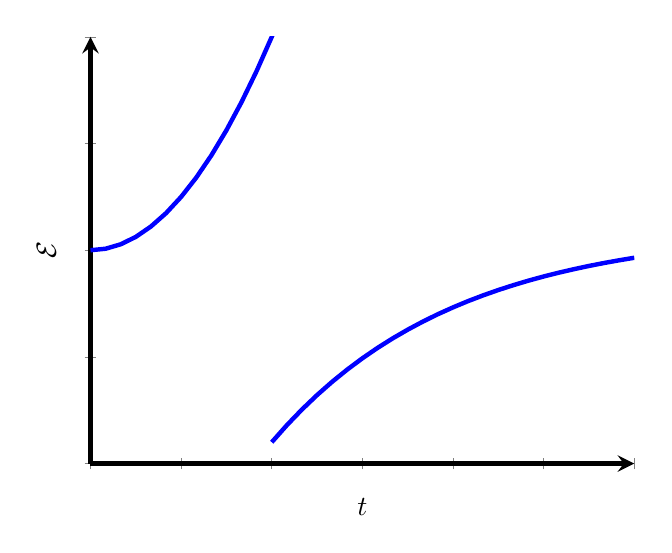
\begin{tikzpicture}[scale=1, transform shape]
				\begin{axis}
					[
						yticklabels={,,},
						xticklabels={,,},
						%
						width=0.7\linewidth,
						height=7cm,
						%
						ymin=-10,
						ymax=10,
						%
						xmin=0,
						xmax=30,
						%
						axis y line=left,
						axis x line=bottom,
						axis line style = ultra thick,
						%
						xlabel={$t$},
						ylabel={$\mathcal{E}$}
					]
					\addplot
						[
							domain={0:20},
							blue,
							ultra thick
						]
						{0.1*x^2};
					\addplot
						[
							domain={10:30},
							blue,
							ultra thick
						]
						{1-10*e^(-0.1*(x-10))};

					%\coordinate (inicioPlano) at (20,128);
					%\coordinate (inicioPlanox) at (20,0);
					%\coordinate (inicioPlanoy) at (0,128);

					%\draw[gray, dashed] (20,128) -- (0,128);

					%\draw[gray, dashed] (20,128) -- (20,0);
					%\draw[gray, dashed] (30,128) -- (30,0);

					%\node (algo) at (9,100) {$I=0.32t^2$};
					%\draw (algo.south) -- ++(-45:8);

					%\node (algo2) at (25,60) {$I=128$};
					%\draw (algo2.north) -- ++(0,55);

					%\node (algo3) at (45,120) {$I=- \frac{32t}{5} +320$};
					%\draw (algo3.south) -- ++(-135:12);
				\end{axis}
			\end{tikzpicture}
		\end{figure}
\end{enumerate}

\textbf{
	Se muestra el perfil de una espira conductora que gira uniformemente alrededor
	de un eje perpendicular al plano del papel.
}
\begin{figure}[H]
	\centering
	\begin{tikzpicture}[scale=1, transform shape]
		\coordinate (A) at (-1.75, 1.5);

		\draw (A) -- ++(-35:3);
		\draw[dashed] (A) -- ++(0,{sin(-35)*3});

		\draw[->] (-2,1) -- (2,1) node [pos=0.975, above=0.1cm] {$\vec{B}$};
		\draw[->] (-2,0) -- (2,0);

		\coordinate (A) at (4,0.5);
		\draw (A) -- +(135:1);
		\draw (A) -- +(225:1);
	\end{tikzpicture}
\end{figure}
\begin{enumerate}[label=\alph*)]
	\item Analiza el flujo magnético antes, después y en el instante que la
		espira se coloque en forma vertical.
		\subitem Subiendo, en máximo y bajando respectivamente.
	\item Analiza el sentido de la corriente inducida para el observador antes y
		después que la espira pase por el eje vertical.
		\subitem Horario, nulo y antihorario.
\end{enumerate}

\textbf{
	\boldmath
	Se tiene una espira metálica dentro de un campo magnético uniforme de
	$0.5T$.
}
\tikzset
{
	equis/.pic =
	{
		%\node at (0,0) {\texttt{x}};
		\foreach \t in {45, 135, 225, 315}
		{
			\draw (0,0) -- (\t:0.125);
		}
	}
}
\begin{figure}[H]
	\centering
	\begin{tikzpicture}[scale=1, transform shape]
		\draw (0,0) circle (2);
		\foreach \x in {0, ..., 5}
		{
			\foreach \y in {0, ..., 5}
			{
				\pic at(\x-2.5,\y-2.5) {equis};
			}
		}
		\draw (-2.5, 2.5) circle (0.2) node [above=0.2cm] {$\vec{B}=cte$};
	\end{tikzpicture}
\end{figure}

\begin{enumerate}[label=\alph*)]
	\item Determina la fuerza electromotriz inducida y el sentido de la
		corriente inducida, si la espira empieza a dilatarse a razón de
		$8 \frac{cm^2}{s} $
		\begin{align*}
			|\mathcal{E}| &= \frac{d\phi}{dt}\\
			\\
			\frac{d\phi}{dt} &= 0.5T* 0.0008 \frac{m^2}{s} * \cancel{\cos{90°}}\\
			\\
			|\mathcal{E}| &= 4*10^{-4}V
		\end{align*}
		Antihorario
	\item Determina la fuerza electromotriz inducida y el sentido de la
		corriente inducida, si la espira empieza a encogerse a razón de
		$10 \frac{cm^2}{s} $
		\begin{align*}
			|\mathcal{E}| &= \frac{d\phi}{dt}\\
			\\
			\frac{d\phi}{dt} &= 0.5T* 0.001 \frac{m^2}{s} * \cancel{\cos{90°}}\\
			\\
			|\mathcal{E}| &= 5*10^{-4}V
		\end{align*}
		Horario
\end{enumerate}

\vfill
Código fuente: \url{https://github.com/otreblan/fisi-2-tarea-7}

\end{document}
%}}}
